\documentclass[useAMS,usenatbib,a4paper]{mn2e}
\usepackage{graphicx}
\usepackage{aas_macros}
\usepackage{multirow}
\usepackage[draft]{hyperref} % draft option seems to fix some hyperref issues
\usepackage{subfigure}
     \voffset=-0.8in
     
\title[Mid-Infrared Spectroscopy of M31]{Mid-Infrared Spectroscopy of the Andromeda Galaxy}
\author[D. Hemachandra et al.]
{D. Hemachandra$^{1}$\thanks{E-mail: dhemacha@uwo.ca},
P. Barmby$^{1}$, 
E. Peeters$^{1}$, 
S.P. Willner$^{2}$, 
M.L.N. Ashby$^{2}$,
H.A. Smith$^{2}$, 
\newauthor 
K.D. Gordon$^{3}$,
D.A. Smith$^{3}$,
and
G.G. Fazio$^{2}$\\
$^{1}$Department of Physics and Astronomy, University of Western Ontario, London, ON, N6A 3K7, Canada\\
$^{2}$Harvard-Smithsonian Center for Astrophysics, Cambridge, MA 02138, USA\\
$^{3}$Space Telescope Science Institute, 3700 San Martin Drive, Baltimore, MD 21218, USA
}


\begin{document}

\date{}

\maketitle

\label{firstpage}

% MLNA comments
% PB: actually, I think these are all dealt with.


\begin{abstract}
We present {\sl Spitzer}/Infrared Spectrograph 5--21~$\mu$m spectroscopic maps towards 12 regions in the Andromeda galaxy (M31). 
These regions include the nucleus, bulge, an active region in the star-forming ring, and 9 other regions chosen to cover a range of mid-to-far-infrared colours. 
PAH feature ratios (6.2~$\mu$m and 7.7~$\mu$m features compared to the 11.3~$\mu$m feature) 
measured from our extracted M31 spectra are consistent with these seen in other nearby galaxies. 
Our  observations did not recover the unusual PAH ratios (suppressed 6--8~$\mu$m features and an enhanced 11.3~$\mu$m feature) seen in 
spectro-imaging observations with the ISOCAM instrument on the Infrared Space Observatory. 
The equivalent widths of the main PAH 
features decrease with increasing radiation hardness, consistent with that observed for other nearby spiral and starburst galaxies. 
The nucleus does not show any PAH emission except for the 11.3~$\mu$m feature, but does show strong silicate emission at 9.7~$\mu$m. 
Both of these characteristics provide evidence for a low luminosity active galactic nucleus in M31.
\end{abstract}

\begin{keywords}
galaxies: individual: M31 --
galaxies: ISM --
galaxies: nuclei --
infrared: ISM --
ISM:  molecules -- 
ISM: lines and bands
\end{keywords}



\section{Introduction}

Mid-infrared spectra provide a unique diagnostic tool to understand the physical conditions in the interstellar medium of galaxies. 
The rich range of spectral features (Polycyclic Aromatic Hydrocarbons (PAHs), atomic fine structure lines (e.g. Ne, S) and the
amorphous silicate feature centred at 9.7~$\mu$m) provide information on dust properties, radiation field and star formation. 
With the advent of infrared space telescopes, such as the Infrared Space Observatory (ISO, \citealt{Kessler1996}) and 
the {\em Spitzer} Space Telescope \citep{spitzer2004}, we have been able to well explore the infrared emission from galaxies. 

PAHs are known as the main carrier of the ubiquitous mid-IR emission bands (e.g. \citealt{Allamandola1989}, 
\citealt{Tielens2008}). They are large hydrocarbon molecules consisting of $\sim$50--100 carbon atoms. 
The main PAH features are seen at 3.3, 6.2, 7.7, 8.6, 11.3 and 12.7~$\mu $m (e.g.\citealt{Mattila1996}, \citealt{Peeters2002}), 
and these bands are due to the vibrational de-excitation of PAH molecules  through bending and stretching modes of C-H and C-C bonds \citep{Tielens:2005lr}. 
The 6 to 8 micron features are thought to originate mostly from ionized PAHs and the 3.3, 11.3, 12.7 and 17.1~$\mu$m 
emission bands from neutral PAHs \citep{Peeters2002}. 


The relative strengths of the PAH features do not vary much within normal-luminosity galaxies \citep{Smith:2007lr} or within 
massive starburst galaxies \citep{Brandl2006}. But they do change significantly close to active galactic nuclei where the 
strength of PAHs gets weaker (\citealt{Roche1991}, \citealt{Smith:2007lr}). \citet{Smith:2007lr}  found that the mid-IR 
spectra from weak AGNs show suppressed 6 to 8~$\mu$m PAH features but are bright at 11.3~$\mu$m. 
A possible explanation for this behaviour is that AGNs alter the grain composition by selective destruction of small ionized PAHs. 
ISOCAM spectro-imaging observations of M31\citep{1998Cesarsky} showed that four regions including the nucleus and bulge 
of this galaxy have very odd PAH spectra, bright at 11.3 and 12.7~$\mu$m but lacking the usual 6.2, 7.7, and 8.6 micron bands. 
Investigating this unusual PAH emission was the main motivation for the work described in this paper. 


Previous studies of nearby galaxies indicate that metallicity and radiation hardness correlate with PAH equivalent widths (EQWs). 
\citet{Smith:2007lr} and \citet{Engelbracht_2008} showed that PAH EQWs in nearby star forming galaxies  decrease with increasing radiation hardness. 
But  \citet{Brandl2006} found no correlation within their starburst sample.  With metallicity, PAH EQWs show an anti-correlation 
in star-forming galaxies \citep{Marble_2010}. This variation of PAHs among galaxies has also been observed within H~{\sc ii} regions 
of a single galaxy (M101) by \citet{Gordon:2008lr}. But there are no other investigations done on a single star-forming galaxy with 
sufficiently high resolution to see whether the correlations mentioned above hold within a galaxy similar to the Milky Way.


The amorphous silicate feature at 9.7 $\mu$m is another aspect of the mid-IR spectra of galaxies. Depending on the presence of silicate 
absorption or emission, the overall shape of the mid-IR spectra, that is the continuum and the PAH intensities, can change. \citet{Spoon2007} 
classified infrared galaxies based on the equivalent width of the 6.2 $\mu$m PAH feature and the strength of the 9.7 $\mu$m silicate feature. 
They  found galaxies spread along two distinct branches: one of AGN and starburst-dominated spectra and one of deeply obscured 
nuclei and starburst-dominated spectra. The first branch is horizontal along emission or weak-absorption of the silicate feature and show no 
correlation with the 6.2~$\mu$m PAH feature (Figure~1 in \citet{Spoon2007}). Silicate emission at 9.7~$\mu$m has also been observed in both 
Seyfert~1 and Seyfert~2 galaxies \citep{Mason2009}. Therefore it is important to study the infrared spectra from nuclei with higher resolution 
to understand this silicate feature and how it reflects the physical structure of the nucleus. 

M31 with its proximity ($\sim$780 kpc) and rich observational databases provides the most detailed view of a star forming galaxy similar 
to the Milky Way. The active star forming ring \citep{Barmby2006lr} provides evidence of abundant PAHs in M31. 
We employed mid-IR spectral maps from the {\em Spitzer}/Infrared Spectrograph (IRS) from 12 regions of M31 for a further investigation of 
its infrared properties. This sample includes the nucleus, bulge, an active region in the star-forming ring (all previously observed by ISOCAM), and 9 
other regions chosen to cover a range of properties as described in Section~\ref{sect:irs_obs}. 
We obtained the processed version of ISOCAM observations of M31 and compare them with the IRS results in Section~\ref{sect:iso_vs_irs}. 
Section~\ref{sect:pah_ratios} discusses PAH intensity ratios.
In Section~\ref{sect:eqw_rh}, we investigate the relationship between PAH equivalent widths and radiation 
hardness and compare to that found by \citet{Engelbracht_2008} and \citet{Gordon:2008lr}. Metallicity and PAH EQWs are compared in 
Section~\ref{sect:eqw_met}, and Section~\ref{sect:nucleus} discusses the dust properties of the nucleus. 	



\section{Observations and Data Reduction}

\subsection{IRS observations}
\label{sect:irs_obs}

% SPW: Fig 1: label F_nu(8 \micron), etc., not just "8/24".
\begin{figure}
\centering
\includegraphics[width = 8 cm]{./colormaps.png}
\caption{$8 - 24/70 - 160$ $\mu$m colour-colour diagram of M31 obtained from IRAC and MIPS. The plot is divided into 9 regions (black grid) and the observations were made to cover those regions. The triangles indicate the regions we observed. ({\bf Needs a better explanation} )}
\label{colourmaps}
\end{figure}

We obtained mid-infrared spectral maps of 12 regions in M31 using the {\em Spitzer}/IRS instrument \citep{IRS2004} covering wavelengths from 5 to 21 microns. 
These regions include the nucleus, two regions previously observed by ISOCAM, and 9 other regions chosen to cover a range of UV intensities, 
metallicities and dust temperatures. Dust temperatures were determined using an $8 - 24/70 - 160$ $\mu$m colour-colour diagram 
(see Figure~\ref{colourmaps}). The locations of the observed regions are shown in Figure~\ref{m31}, and 
their coordinates are given in Table~\ref{regions}. The two regions previously observed by ISOCAM are the region from the bulge and the 
region from the active region in the star-forming ring (Region 9 in our sample). A background observation was also made off the galaxy 
along the minor axis and it was used to enable the background subtraction from the data cubes.

% SPW: Table 1: mark (with a footnote) the regions that have ISO data.
%MLNA: Table 1 would be better if it included the galactocentric radii (perhaps), and the UV intensities, metallicities, and dust temperatures (definitely) used to choose them as targets in the first place.  Also which fields were previously observed by ISO/ISOCAM.  Suggested new title: Spitzer/IRS Target Locations in M31.

%SPW: As to tables, I'd consolidate 1, 2, and 5 into a single table.  Add rows as appropriate for "nucleus" and "north", and give their dimensions in a footnote.  
\begin{table}
 \centering
 \begin{minipage}{70mm}
\caption{IRS Targets and their metallicities in M31
\label{regions}}
  \begin{tabular}{lccc}
  \hline Name & R.A. & Decl. &$12+\log({\rm O/H})$
   \\
 \hline
 Nucleus$^a$&00:42:44.31&41:16:09.4& - - -\\
Bulge$^a$&00:42:35.00&41:21:01.0&$8.90\pm0.03$\\
Region 1&00:41:30.41&40:43:07.8&$9.20\pm0.20$\\
Region 2&00:45:22.85&41:38:53.1&$9.07\pm0.02$\\
Region 3&00:40:37:37&41:01:29.4&$8.85\pm0.01$\\
Region 4&00:41:17.86&41:07:09.8&$8.89\pm0.06$\\
Region 5&00:43:39.57&41:19:03.1&\hspace{0.14cm}$8.93\pm0.08$$^b$\\
Region 6&00:43:35.72&41:23:15.0&$8.73\pm0.08$\\
Region 7&00:40:53.98&40:58:58.9&$8.40\pm0.08$\\
Region 8&00:42:21.60&41:07:17.4&\hspace{0.14cm}$8.94\pm0.08$$^b$\\
Region 9$^a$&00:41:00.00&40:36:20.3&$8.86\pm0.02$\\
NGC206&00:40:20.20&40:44:54.0& - - -\\
Background&00:44:41.8&40:58:56.0& - - -\\
\hline
\end{tabular}
{$^a$Regions that have ISOCAM data. 
$^b$Metallicity values obtained from the radial metallicity profile of M31.}
\end{minipage}
\end{table}

\begin{figure*}
\centering
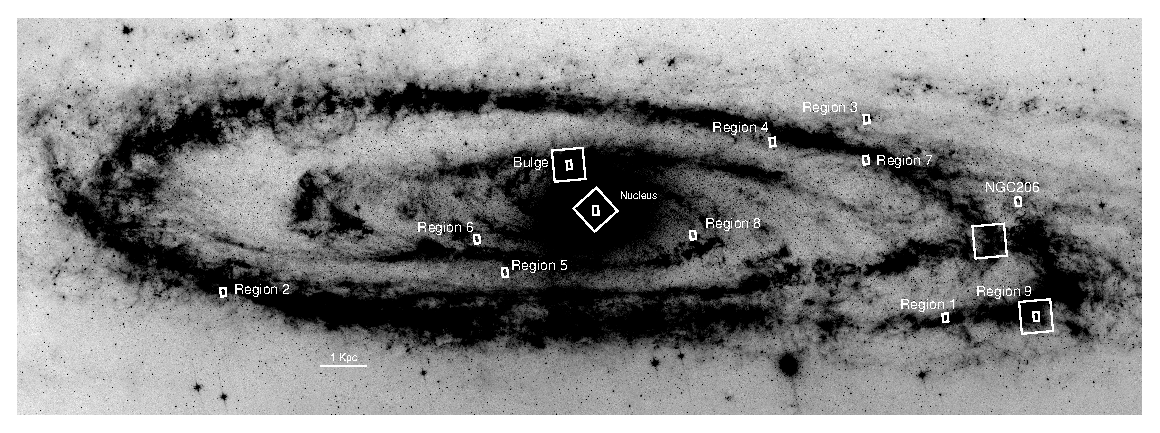
\includegraphics[scale=0.9]{./m31_map.eps}
\caption{An 8 micron IRAC image of M31 \citep{Barmby2006lr}. Small white rectangles ($30\arcsec\times50\arcsec$) show the regions that we observed and larger squares ($192\arcsec\times192\arcsec$) show the regions observed by  \citet{1998Cesarsky}.
\label{m31}
}
\end{figure*}

% SPW: Probably no need to mention LL1, which wasn't used.
For our observations we used the Short-Low (SL) and Long-Low (LL) modules which cover wavelengths from 5 to 21 microns. 
The Low modules have resolving power changing 60--130. Each low-resolution module is divided into two sub-slits 
which provide spectroscopy in either first or second order. They are denoted as SL1 (7.5--14.5~$\mu$m), SL2 (5.2--7.6~$\mu$m),
LL1 (20.5--38.5~$\mu$m), and LL2 (14.5--20.75~$\mu$m).

All regions were observed in September 2007 (PID 40032) with both orders of the Short-Low module (SL2, SL1) and the Long-Low order LL2. 
The Long-Low order LL1 was not used for observations because this spectral region contains few features. The map size was based on the size 
of the IRS slits (SL: $3.6\arcsec \times 57\arcsec$, LL: $10.5\arcsec \times 168\arcsec$). Each region was covered by 18 overlapping observations 
of the SL slit and 11 overlapping observations of the LL slit making the map size $32\arcsec \times 57\arcsec$ for SL and $58\arcsec \times 168\arcsec$ for LL. 
Figure~\ref{slits} shows an example of the slit arrangement. For the brighter regions (nucleus, bulge), ramp times of 14 s (SL) and 30 s (LL) were used, 
while for the fainter regions, ramp times of 60 and 120 s were used respectively. Background observations were taken with each module (2 per ramp time). 
Since all of the targets are in the same part of the sky, a common background observation was used for multiple targets to subtract the background emission. 

% SPW:  I don't really understand this figure or why it's needed.  Is the point that the SL and LL slits don't align?  You could say that in text and omit the figure.  Alternatively, the figure might make sense with a better caption.  Why two SL regions, for example?
\begin{figure}
\centering
\includegraphics[scale=0.3]{./cubeslits.eps}
\caption{SL1 data cube from the nucleus showing the arrangement of slits used to cover the region. 
Black boxes outline the footprints of the SL1 and the green box outlines the LL2. Blue and red slits show how 
each mode was covered using overlapping slit positions.
\label{slits}
}
\end{figure}

\subsection{IRS Data Reduction}

% SPW: it seems obvious, but it might be worth an explicit mention that all the IRS maps cover additional area than is considered here.
The data were reduced through the SSC pipeline (ver. S17.2.0) and the maps were assembled using the CUBISM program \citep{Smith:2007fk}. 
Bad pixel removal was also done using CUBISM and the background observations were used to subtract the background emission from these cubes 
following the method outlined in \citet{Gordon:2008lr}. Spectra were extracted using a $30\arcsec\times50\arcsec$   rectangular aperture. 
The aperture size was selected to cover the whole overlapping area of the SL and LL modes.

After the spectral extraction there was a noticeable mismatch between the spectra from the SL1 and LL2 modules. To combine all spectra to obtain one spectrum, 
first a photometric comparison was conducted between the IRS spectra and the IRAC 8 micron image of M31 \citep{Barmby2006lr}. For more details 
about this method see the IRAC Instrument Handbook Section 4. An aperture with the same size was used to extract flux from the same regions 
in the IRAC 8 micron image. The photometric calibration of the IRAC is tied to point sources measured within a standard aperture with a radius of 12\arcsec. 
For extended sources,  an aperture correction has to be conducted as mentioned in the IRAC instrument handbook. Therefore an extended source 
aperture correction of 0.824 was applied for all the extractions from the 8 $\mu$m image. The uncertainty value of the IRAC image was estimated 
by taking the standard deviation of pixels values within an aperture of the same size from a position off M31 (00:48:58.00, +42:14:54.00).

% SPW: the color correction factor needs a bit of explanation. Isn't it simply the actual IRS spectrum integrated over the IRAC band's responsivity?  The key thing in the IRAC handbook should be the responsivity curves, not the method.  Just which data did you integrate?  I'd have expected it to be SL2 because otherwise the break between SL1 and SL2 is in the middle of the IRAC filter.  Anyway, some clarification is needed here about exactly what you did.
Then we stitched the SL1 and SL2 using the overlapping regions and applied a colour correction factor $K$, which is a multiplicative factor that 
converts the intensity of an IRS spectrum at a given wavelength to the intensity of an IRAC image taken at the same wavelength. We used the IDL 
code provided by the instrument handbook to compute these $K$ values for all the regions. colour correction values and the corresponding IRS 
data along with the IRAC data are given in Table~\ref{colourK}.

% SPW: Table 2: headers should clarify the difference between IRS specific intensity measured at 8.00 microns (if that's what it is) and IRAC specific intensity measured over the broader bandwidth.  I'd suggest "at 8.00~\micron" for the former and "in 8~\micron\ band" for the latter, but perhaps you can do better.  Using footnotes might be a good alternative.
%
%MLNA: Table 2 should make explicit that the fluxes given are prior to color-correction

\begin{table}
 \centering
 \begin{minipage}{90mm}
\caption{Matched aperture photometry}
  \begin{tabular}{lcccc}
  \hline{Name}&{IRS Intensity}&{IRAC Intensity}&{colour K$^b$}&{x$^{a,}$ $^c$} \\ {}&{at 8 $\mu$m$^a$}&{at 8 $\mu$m$^a$}&{}&{} 
   \\
 \hline
 Region 1 & 1.8505 & 1.3923 & 0.532 & 0.3061
 \\ Region 2  & 1.8238 & 1.3731 & 0.555 & 0.2148
 \\ Region 3 & 0.7192 & 0.9689 & 0.767 & 0.3218
 \\ Region 4 & 1.1431 & 0.8513 & 0.589 & 0.0407
 \\  Region 5 & 0.6787 & 0.8088 & 0.773 & 0.1834
 \\  Region 6  & 0.6399 & 0.7656 & 0.927 & 0.0479
 \\  Region 7  & 1.1538 & 0.8243 & 0.526 & 0.1380
 \\ Region 8 & 0.5556 & 0.7135 & 0.877 & 0.1148
 \\  Region 9 & 1.9413 & 1.6562 & 0.606 & 0.3107 
 \\ Bulge & 2.6956 & 2.5473 & 0.532 & 1.2425\\
\hline
 \label{colourK}
\end{tabular}\\
 {$^a$Units are MJy~sr$^{-1}$. 
 $^b$Colour correction factors 
 $^c$Offset between IRAC and IRS as mentioned in eq. 1. Intensities are given prior to the extended source correction and the colour correction.}
\end{minipage}
\end{table}

% SPW: it isn't clear to me exactly how you estimated the IRAC uncertainty.
%Eq 1: because the IRAC uncertainties are much smaller than the IRS ones, you have to use the IRAC intensities as the independent variable (unless you take uncertainties on both axes into account in the fitting).  This probably won't change the answer much, but it might.

%MLNA: How was the line of best fit derived -- did you weight by uncertainty?
%
Figure~\ref{offset} compares the IRS and IRAC 8~$\mu$m photometry. The line of best fit wighted by the uncertainties has a slope of $0.81\pm0.08$ 
and intercept of $-0.05\pm0.06$.  Since the intercept in Figure~\ref{offset} is not zero with a higher uncertainty, it can be concluded that the offsets 
between orders are due to an additive offset than a multiplicative offset. Also an additive offset favours more for stitching SL and LL modes. 
Based on this argument, first we shifted the combined SL1 and SL2 spectrum so that the intensity at 8 $\mu$m matches with that of IRAC 8 micron image. 
To do this shift, the following equation was used to find the offset values ($x$) between IRS and IRAC image intensities at 8 microns. 
\begin{equation}
F_{IRAC8} = [ F_{IRS8} + x ] \times K
%K is the colour correction factor.
\end{equation}
\footnotesize
%\emph{Where K is the colour correction factor, Flux$_{IRAC8}$ is the flux of the IRAC 8 $\mu$m image, Flux$_{IRS8}$ is the flux of IRS spectra at 8 $\mu$m and x is the offset.}
\normalsize
$K$ is the colour correction factor, F$_{IRAC8}$ is the intensity of the IRAC 8 $\mu$m image (aperture corrected) and F$_{IRS8}$ is the intensity of IRS spectra at 8~$\mu$m. 
The offsets for all the regions are listed in Table \ref{colourK}. After that the LL2 mode was stitched by shifting it towards the SL1 by an amount of the average difference in their overlapping spectral regions.	
% SPW: Sec 2.2 par 5: clarify that "stitched to" means via an additive constant for each spectrum.
%MLNA Can you cite others who applied *offsets* to force IRS spectra to match up, as opposed to using only multiplicative factors -- is this standard practice?
%

	
\begin{figure}
\centering
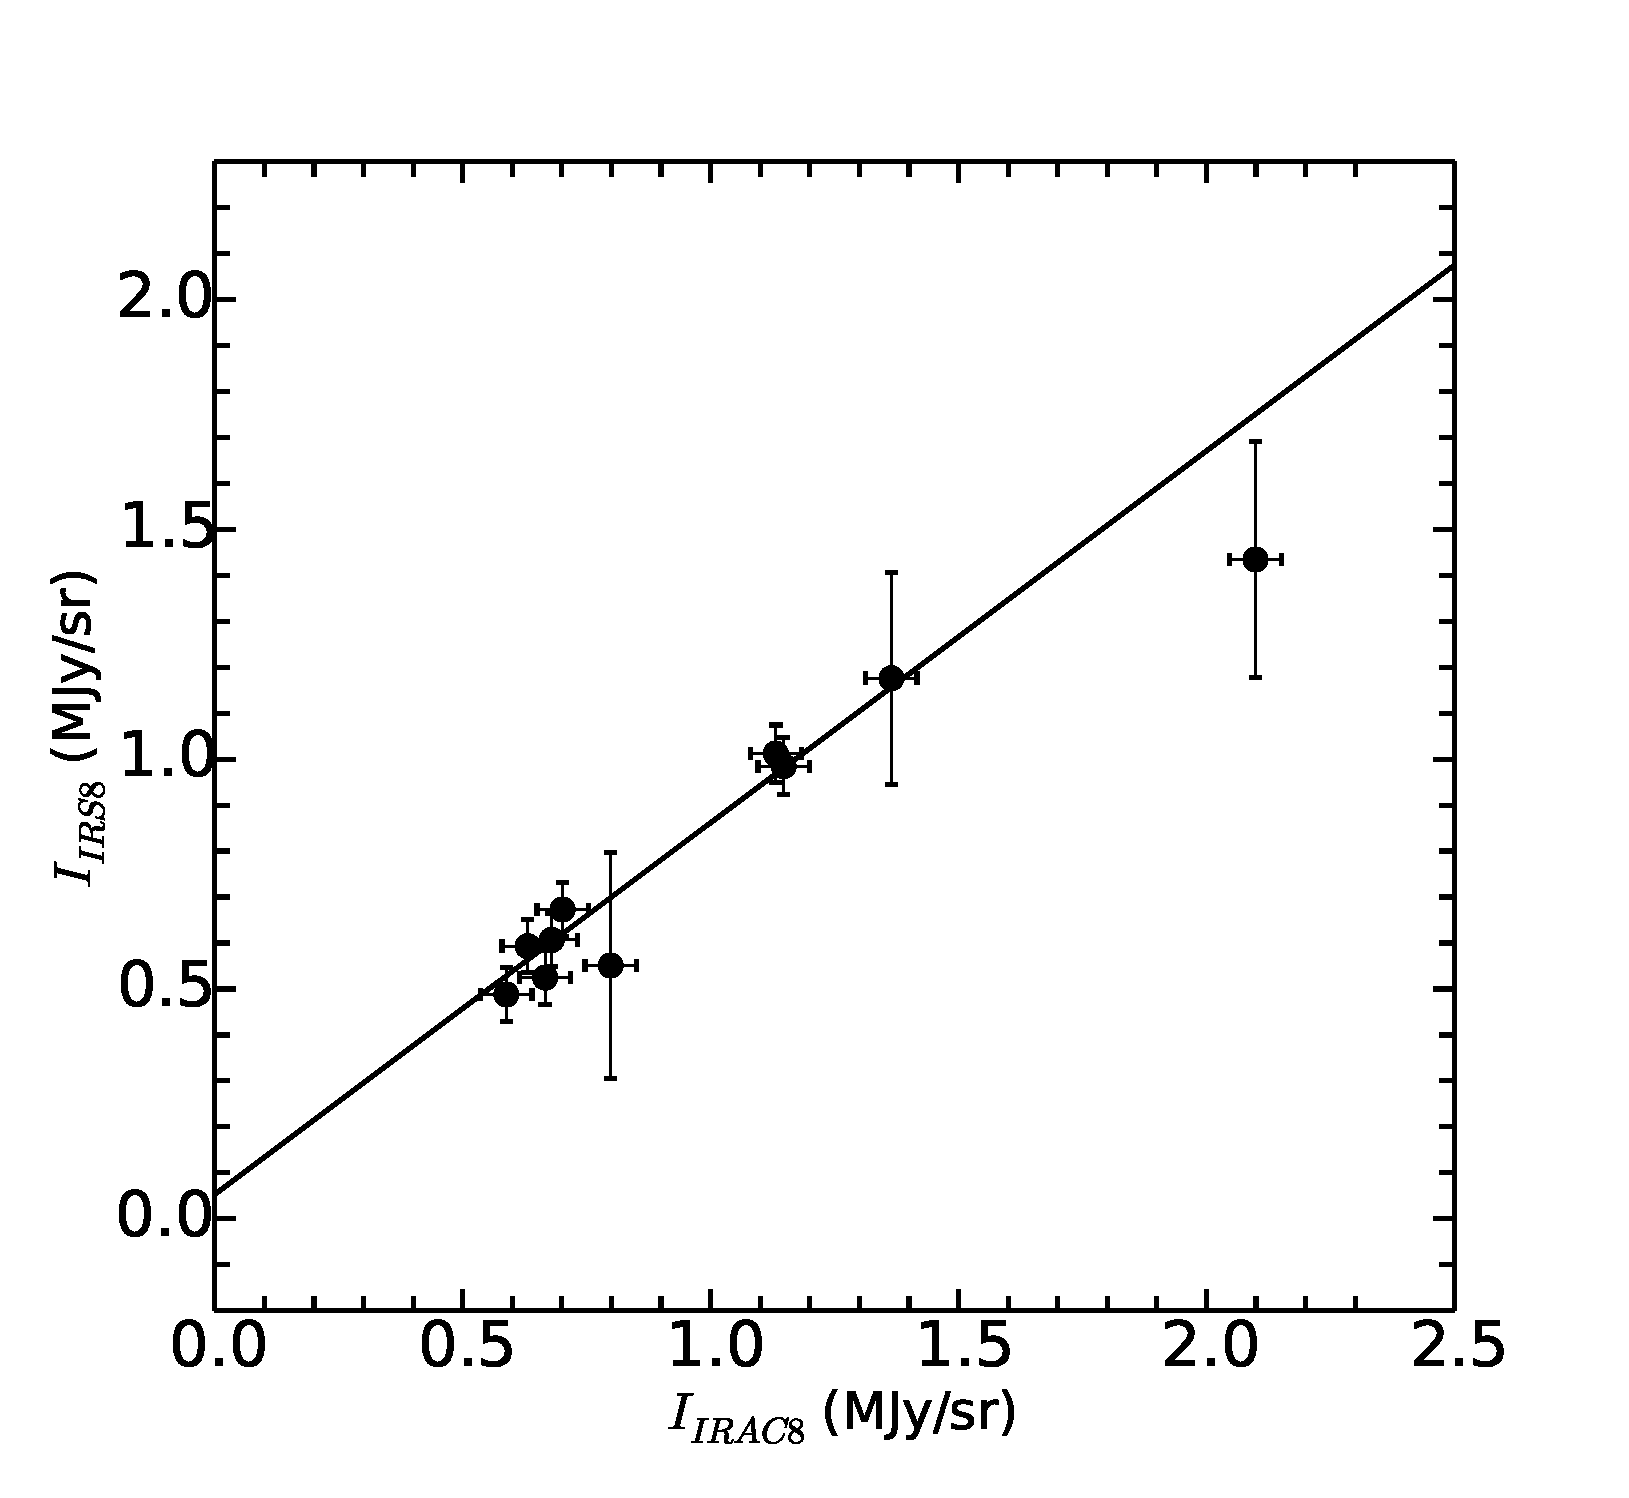
\includegraphics[scale=0.25]{./offset.eps}
\caption{ Intensity of the aperture corrected IRAC 8~$\mu$m image vs that of the colour corrected IRS spectra at 8~$\mu$m  obtained using the same aperture for our regions in M31. The straight line is the line of best fit. }
\label{offset}
\end{figure}

% TODO: tables need some reformatting, such as $x\pm y$

\begin{table*}
 \centering
 \begin{minipage}{200mm}
\caption{PAH Emission Line Strengths$^a$}
  \begin{tabular}{l c c  c  c  c  c  c  c  c  c c }
  \hline {Region  }&{5.7$\mu$m  }&{6.2$\mu$m  }&{7.7$\mu$m  }&{8.3$\mu$m  }&{8.6$\mu$m  }&{10.7$\mu$m  }&{11.3$\mu$m  }&{12.0$\mu$m  }&{12.7$\mu$m  }&{17.0$\mu$m  } 
   \\
 \hline
 Region 1 &$10\pm1$            & $34\pm1$        & $107\pm10$        & $13\pm1$       & $14.1\pm0.9$        & $2.2\pm0.3$        & $33.4\pm0.9$        & $9.1\pm0.5$        & $16\pm1$        & $17\pm1$        \\
Region 2 &$7.7\pm0.9$        & $31.2\pm0.8$        & $106\pm8$        & $9\pm1$           & $19.8\pm0.8$        & $1.5\pm0.2$        & $32.0\pm0.8$        & $6.6\pm0.4$        & $15\pm1$        & $14.7\pm0.9$        \\
Region 3 &$8\pm4$              & $25\pm3$                & $111\pm22$       &$21\pm4$       & $7\pm3$                 & $1.1\pm0.9$        & $19\pm3$             & $6\pm1$             & $14\pm3$           & $13\pm2$        \\
Region 4 &$4\pm1$              & $15.8\pm0.9$        & $59\pm9$        & $7\pm1$           & $11.6\pm0.8$          & $0.8\pm0.2$        & $19.9\pm0.8$        & $3.5\pm0.4$        & $9\pm1$             & $12.5\pm0.9$        \\
Region 5 &$1\pm1$              & $7\pm1$                 & $22\pm3$        & $3\pm1$           & $5.8\pm0.8$            & $0.9\pm0.2$        & $12.7\pm0.8$        & $2.4\pm0.4$        & $6.3\pm0.4$        & $10\pm2$        \\
Region 6 & - - - -                      &$ 7.3\pm0.9$         & $22\pm7$        & $3\pm1$            & $3.6\pm0.8$       & $0.8\pm0.2$        & $10.8\pm0.8$        & $1.9\pm0.4$        & $4.5\pm0.4$        & $8.3\pm0.6$        \\
Region 7 &$5.9\pm0.9$        & $17.7\pm0.9$       & $57\pm8$        & $9\pm1$            & $12.8\pm0.8$        & $1.6\pm0.2$        & $21.8\pm0.8$        & $5.2\pm0.4$        & $11\pm1$             & $13\pm2$        \\
Region 8 &$2.\pm1$              & $3\pm1$              & $6\pm3$            & $3\pm1$            & $2.7\pm0.8$        & $1.4\pm0.3$        & $4.4\pm0.8$            & - - - -                      &  - - - -               & $4.1\pm0.7$        \\
Region 9 &  - - - -                     & $38\pm3$          & $133\pm29$        & $25\pm4$        & $15\pm3$            & $2.4\pm0.8$        & $37\pm3$               & $14\pm1$             & $25\pm3$        & $19\pm6$        \\
Bulge       & - - - -                       & $38\pm2$           & $219\pm27$        & $32\pm4$        & $20\pm3$           & $2.0\pm0.9$        & $53\pm3$              & $14\pm1$           & $29\pm3$        & $39\pm2$       \\
\hline
 \label{PAHlinetable}
\end{tabular}\\
{$^a$Units are 10$^{-9}$~W~m$^{-2}$.}
\end{minipage}
\end{table*}







\begin{table*}
 \centering
 \begin{minipage}{200mm}
\caption{PAH Emission Line Equivalent Widths$^a$}
  \begin{tabular}{l c c  c  c  c  c  c  c  c  c c }
  \hline {Name  }&{5.7$\mu$m  }&{6.2$\mu$m  }&{7.7$\mu$m  }&{8.3$\mu$m  }&{8.6$\mu$m  }&{10.7$\mu$m  }&{11.3$\mu$m  }&{12.0$\mu$m  }&{12.7$\mu$m  }&{17.0$\mu$m  } 
   \\
 \hline
 Region 1 &$0.39\pm0.08$        & $1.2\pm0.1$             & $3.4\pm0.3$        & $0.43\pm0.04$        & $0.47\pm0.04$        & $0.09\pm0.01$        & $1.45\pm0.04$        & $0.43\pm0.03$        & $0.78\pm0.03$              & $1.27\pm0.05$        \\
 Region 2 &$0.28\pm0.04$        & $1.02\pm0.06$        & $3.4\pm0.2$        & $0.32\pm0.04$        & $0.70\pm0.04$        & $0.07\pm0.01$        & $1.58\pm0.04$        & $0.35\pm0.02$        & $0.85\pm0.03$              & $1.35\pm0.06$        \\
 Region 3$^b$ &$4\pm2$           & $8\pm2$                   & $19\pm4$            & $2.8\pm0.8$             & $0.9\pm0.5$             & $0.1\pm0.1$            & $2.1\pm0.3$             & $0.7\pm0.2$            & $1.6\pm0.2$                   & $2.4\pm0.3$        \\
 Region 4 &$0.28\pm0.09$        & $1.0\pm0.1$             & $3.7\pm0.4$       & $0.5\pm0.1$              & $0.77\pm0.07$        & $0.07\pm0.02$        & $1.67\pm0.06$        & $0.31\pm0.04$        & $0.86\pm0.05$             & $1.68\pm0.07$        \\
 Region 5 & - - - -                          & $0.12\pm0.03$        & $0.61\pm0.08$   & $0.10\pm0.03$        & $0.20\pm0.03$        & $0.05\pm0.01$        & $0.77\pm0.03$        & $0.17\pm0.03$        & $0.50\pm0.04$            & $1.6\pm0.2$        \\
 Region 6 & - - - -                          & $0.10\pm0.04$        & $0.6\pm0.2$        & $0.10\pm0.04$        & $0.14\pm0.03$        & $0.05\pm0.01$        & $0.77\pm0.04$        & $0.15\pm0.03$        & $0.42\pm0.04$            & $1.7\pm0.1$        \\
 Region 7 &$0.32\pm0.05$        & $0.86\pm0.06$        & $2.8\pm0.2$        & $0.44\pm0.06$        & $0.69\pm0.06$        & $0.12\pm0.02$        & $1.81\pm0.07$        & $0.48\pm0.05$        & $1.11\pm0.08$            & $2.2\pm0.2$        \\
 Region 8 &$0.03\pm0.04$        & $0.04\pm0.03$        & $0.2\pm0.10$      & $0.09\pm0.04$        & $0.10\pm0.03$        & $0.09\pm0.02$        & $0.30\pm0.02$        & $0.00\pm0.00$        & $0.01\pm0.01$            & $0.62\pm0.07$        \\
 Region 9$^b$ & - - - -                 & $237\pm100$          & $151\pm60$        & $16\pm6$                 & $8\pm3$                   & $0.5\pm0.2$             & $7\pm1$                   & $2.3\pm0.6$             & $3.6\pm0.8$                 & $2.4\pm0.8$  \\
 Bulge       & - - - -                          & $1.2\pm0.2$            & $4.0\pm0.4$        & $0.51\pm0.07$         & $0.30\pm0.06$        & $0.03\pm0.01$        & $0.78\pm0.03$        & $0.22\pm0.02$        & $0.49\pm0.03$            & $1.16\pm0.04$ \\             
\hline
 \label{EQW}
\end{tabular}\\
{$^a$Units are $\mu$m.
%SPW Table 3: fn b _probably_ should be something like "Continuum for these regions is very weak.  Equivalent widths are highly uncertain and not considered in the analysis."
 
$^b$EQWs from these two regions were removed from the analysis (see Section~\ref{sect:data_analysis}).}
\end{minipage}
\end{table*}





%MLNA: Table 5 has names inconsistent with other tables in the paper
% PB: fixed?
\begin{table*}
 \centering
 \begin{minipage}{100mm}
\caption{Atomic Emission Line Strengths$^a$}
  \begin{tabular}{l c c  c  c  c  c  }
  \hline{Name  }&{[Ar~{\sc ii}] }&{[Ar~{\sc iii}]  }&{[S~{\sc iv}]}&{[Ne~{\sc ii}]   }&{[Ne~{\sc iii}]   }&{[S~{\sc iii}]  }\\
{}&{\tiny{7.0$\mu$m} }&{\tiny{9.0$\mu$m }}&{\tiny{10.5$\mu$m}}&{\tiny{12.8$\mu$m  }}&{\tiny{15.5$\mu$m } }&{\tiny{18.7$\mu$m }} 
   \\
 \hline 
 
Region 1 &    $<$15.2                 & $<$16.4                 & $6\pm1$                 & $6\pm1$                 & $<$ 4.2                 & $2.2\pm0.4$                \\
Region 2 &    $5\pm3$                 & $<$ 17.4               & $<$5.1                    & $6\pm1$                 & $<$ 2.9                 & $0.9\pm0.5$                 \\
Region 3 &    $<$42.9                 & $27\pm6$              & $<$ 28.9                & $9\pm3$                 & $6\pm1$               & $4.3\pm0.9$                 \\
Region 4 &    $<$11.2                 & $<$10.0                 & $<$4.4                    & $2\pm1$                 & $0.6\pm0.5$        & $1.3\pm0.5$                 \\
Region 5 &    $4\pm3$                 & $<$6.2                   & $<$ 5.2                 & $<$ 4.2                     & $2\pm1$               & $2\pm1$                 \\
Region 6 &    $7\pm3$                & $4\pm2$                 & $<$ 3.8                 & $2\pm1$                  & $5.4\pm0.5$         & $5.3\pm0.5$                 \\
Region 7 &    $3\pm3$                 & $<$12.6                 & $2.3\pm0.9$        & $10\pm2$                & $<$ 2.9                 & $8\pm1$                \\
Region 8 &    $<$11.8                  & $5\pm2$                & $<$4.9                  & $<$2.6                      & $11.6\pm0.5$     & $6.5\pm0.5$                 \\
Region 9 &    $24\pm10$             & $35\pm8$             & $<$ 2.7                 & $38\pm3$                 & $7\pm4$               & $15.3\pm5.6$                 \\
Bulge &          $10\pm7$               & $49\pm7$              & $<$ 30.4               & $19\pm4$                 & $7\pm2$               & $2\pm1$      \\            

\hline
 \label{Atomic}
\end{tabular}\\
{ $^a$Units are 10$^{-10}$~W~m$^{-2}$. Upper limits are indicated with a $<$ mark.  }
%SPW: Table 4: units of 10^-10 W m^-2 must be wrong.  I'd expect 10^-15 or so.
%How many sigma are the upper limits?

\end{minipage}
\end{table*}



\subsection{ISOCAM Data Reduction}

% SPW:  mention ISO spectral resolution.  I would have preferred to see the ISO FOV and wavelength range mentioned earlier, but I don't see any good place to put them other than here, though the Fig 2 caption is a possibility for the FOV.  Another is a footnote where ISOCAM is mentioned in Sec 2.1 par 1, though I'm not sure ISOCAM should really appear there at all.

To compare our results with previous observations, ISOCAM data of three regions previously observed by \citet{1998Cesarsky} which overlap 
with IRS observations were obtained. We retrieved the highly processed data provided by \citet{Boulanger_F_2005} of these ISOCAM observations. 
The total wavelength range covered was 5.15 to 16.5 $\mu$m and the field-of-view was $32\times 32$ pixels with 6\arcsec\ per pixel. 
An image of the ISOCAM data is shown in Figure~\ref{isonuc}.  For the three regions in common, we extracted spectra using the same aperture as for the IRS data. 

% SPW: Fig 5: mention "negative image" (if that's what it is).  Also mention spectral band of image and the 30x50 box size.
\begin{figure}
\centering
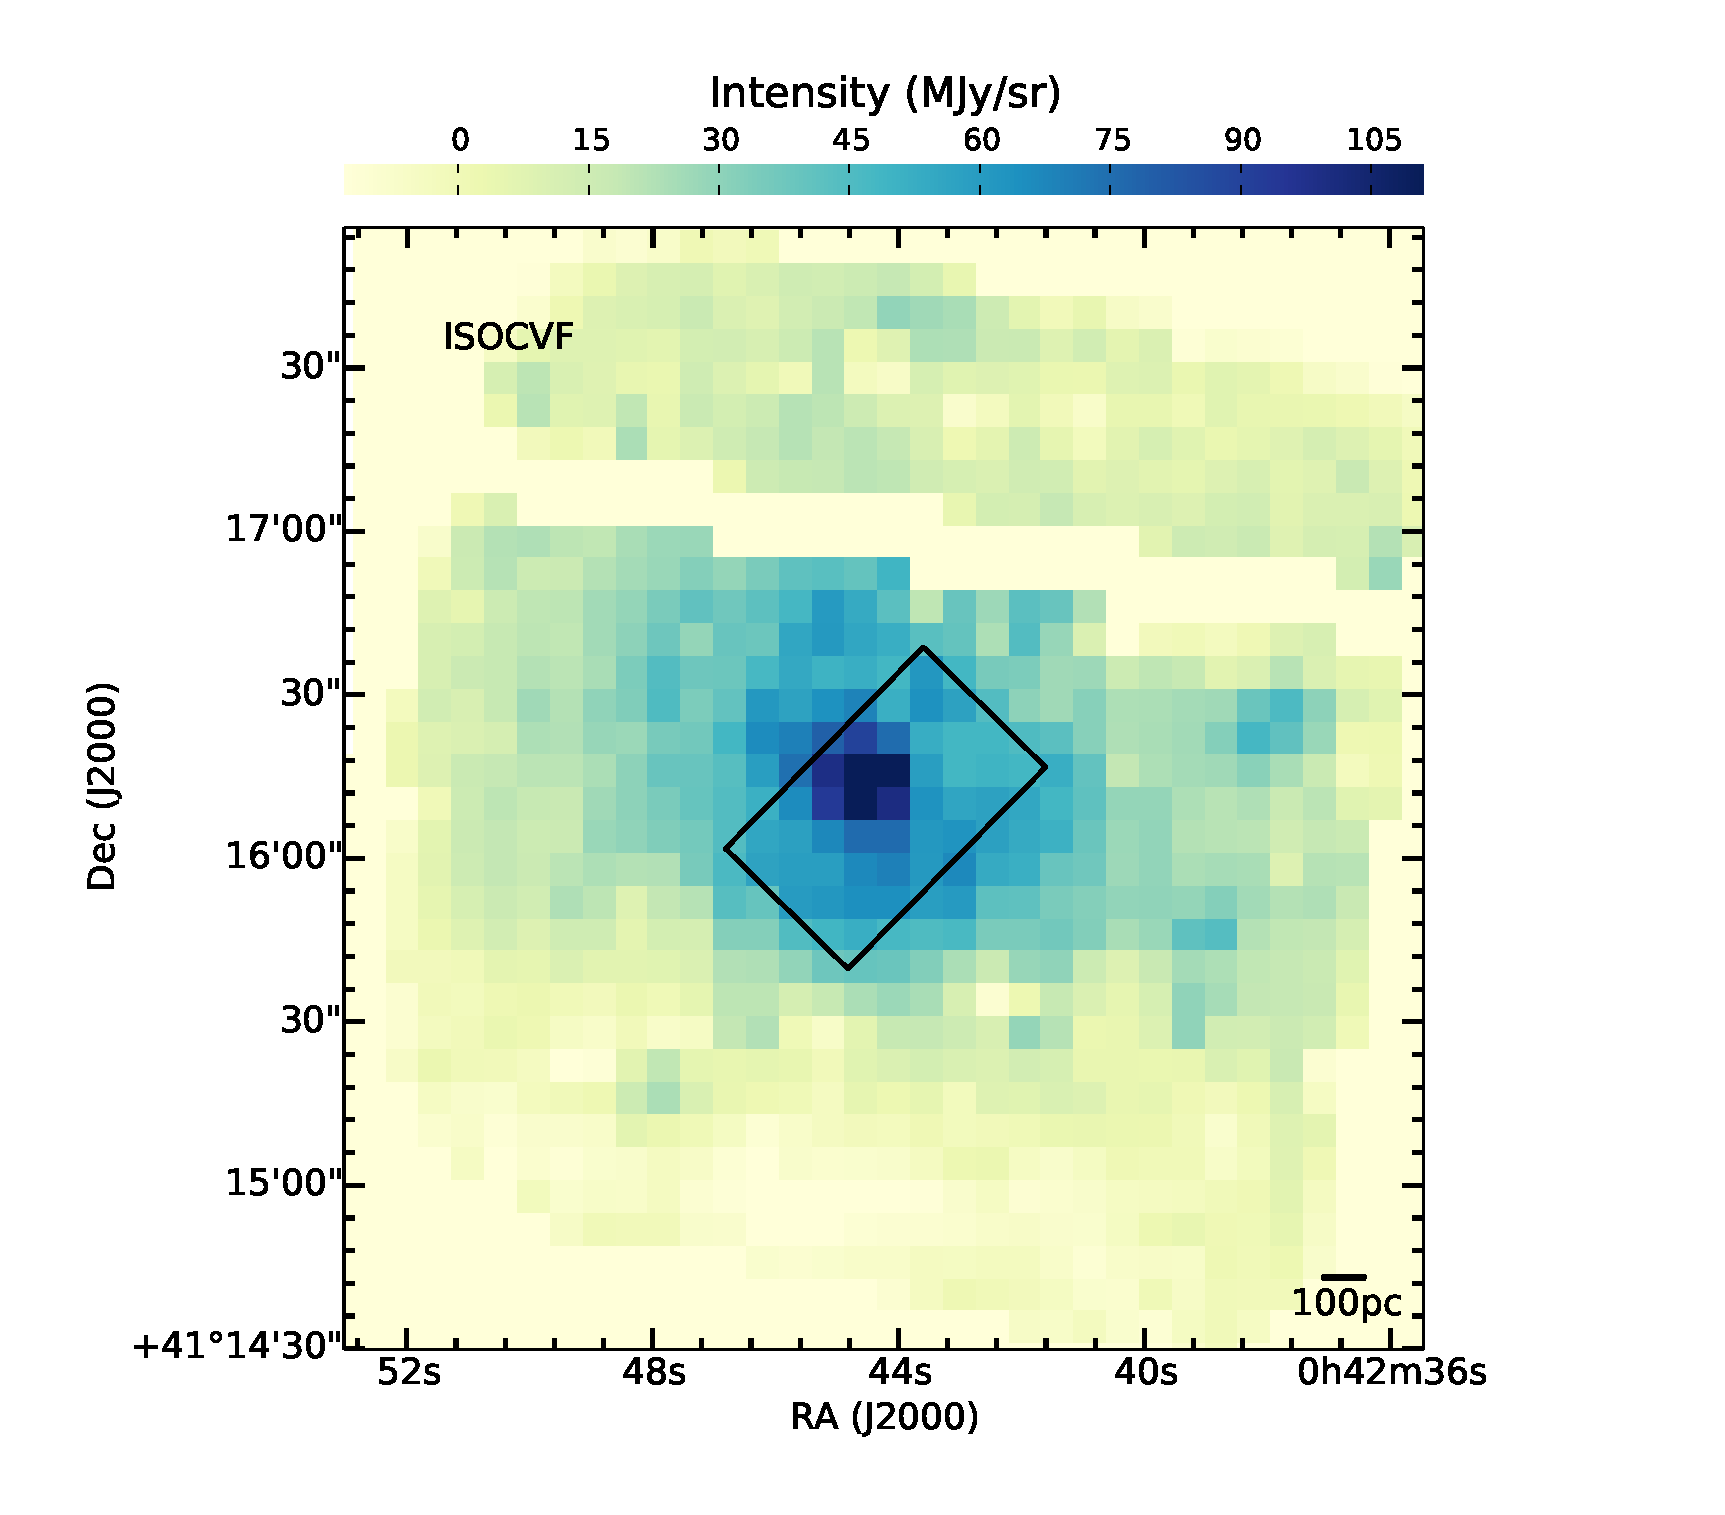
\includegraphics[width = 8cm]{./isonuc.eps}
\caption{11.3~$\mu$m image of the ISOCAM data cube from the nucleus of M31. The black box shows the size of the aperture used to extract spectra.}
\label{isonuc}
\end{figure}



\section{Data Analysis}
\label{sect:data_analysis}

% SPW comments: move to appropriate places
%
%Sec 3 par 2: comment on NGC 206 belongs in Sec 2 and/or note to Table 1. Rest of par belongs later, when dust continuum is discussed.
%
%Sec 3 par 3: belongs later or perhaps omit.
%
%Sec 3.1 par 1: better last sentence "Figure 7 compares ...." Immediately previous reference is Sec 2.3; use \label and \ref to keep these straight.
%
%Sec 3.1 par 2: delete first sentence
%
%Sec 3.1 par 3: if you define ISOxxxx, use those designations.  Remove redundancies.  End with final sentence such as "The new reduction appears to eliminate the discrepancies." Par 4 then isn't needed.
%
%(We should probably plan to send the submitted ms to Diego Cesarsky, but it's too early for that now.)
%
%Sec 3.2 par 1: I don't understand why the last sentence is needed.
%
%Sec 3.2 par 2: generally "modified blackbody" means one with an emissivity varying with wavelength.  I don't think that's what you mean for the stellar spectra.  For the dust spectra, it is likely appropriate, but the form of the variation with wavelength should be given.  I think what you mean in the middle is something like "PAHFIT uses only the minimum number of temperatures needed to fit the data, in most cases two or three for our data."  (What was the maximum number?)
%
%Sec 3.2 par 3: omit "a considerable amount of" or quantify it.  I gather the end result was forcing PAHFIT to set extinction to zero. Also starlight was zero except for the four regions. Basically this par just needs to be terser and more direct.
%
%Sec 3.3 par 1: I'd rephrase "...coming from ordinary dust grains, much larger than PAH molecules."  Omit "Therefore ... M31."  In last sentence, do you mean regions 3 and 9?  Isn't the problem that they have negligible dust continuum, and therefore the EQWs can't be calculated? The feature flux ratios should still be meaningful, though.
%
%Sec 3.4: this is much too long for basically no result.  Unless I'm missing something, the key point is that all the regions are relatively low excitation.  In the one possible exception (6), the [Ne III] flux is based on only a single data point.  I think Table 4 and Fig 10 are fine, but the discussion can be a paragraph.
%
%Table 3: fn b _probably_ should be something like "Continuum for these regions is very weak.  Equivalent widths are highly uncertain and not considered in the analysis."
%
%Table 4: units of 10^-10 W m^-2 must be wrong.  I'd expect 10^-15 or so.
%How many sigma are the upper limits?
%
%General: "Smith et al." are human authors.  Results are given "by" those authors, not "in" them. (Ugh!)


%MLNA: Sec 3 (text) needs to be much clearer as to which spectra (IRS or ISO) are being discussed.

All the main PAH features features, including the 6.2, 7.7, 8.6 and 11.3~$\mu$m bands, are clearly visible in the final processed spectra 
(see Figure \ref{PAHFITplots}) from all the regions except the nucleus. (The spectrum of the nucleus is discussed in Section 4.3.)
They also show atomic line emission such as [Ar~{\sc ii}], [Ar~{\sc iii}], [S~{\sc iii}], [S~{\sc iv}], [Ne~{\sc ii}], [Ne~{\sc iii}] 
and molecular H$_{2}$ emission at 12.3~$\mu$m. Some of the spectra display a contribution to the continuum from starlight emission.

Dust continuum emission from Regions 3 and 9 is very low compared to other spectra and they also show some negative flux values in the shorter 
wavelengths which can be due to instrumental errors. It was observed that the spectrum from the NGC 206 is very noisy, therefore that spectrum 
was removed from our analysis. 


\subsection{ISOCAM versus IRS}
\label{sect:iso_vs_irs}


As mentioned in the Introduction, based on ISOCAM observations \citet{1998Cesarsky} reported a suppression of the common 
6 to 8~$\mu$m features and an enhancement of a broad 11.3 and 12.7 $\mu$m features in four regions of M31. 
In addition, \citet{Pagani_1999} confirmed that the star-forming ring in M31 shows very weak PAH emission in the 6 to 8~$\mu$m region. 
However, the IRS spectra presented here do not show such unusual behaviour (Figure \ref{PAHFITplots}). 
Indeed, except for the nucleus, all regions show a normal mid-IR spectrum similar to other nearby starforming galaxies. 
Therefore, we obtained newly-processed ISOCAM spectra from three regions in our IRS sample (see Section 2.4) 
and compared them with the corresponding IRS spectra (Figure \ref{ISOnIRS}). 
The spectra from both instruments look almost the same. Although the relative intensities of the features in the IRS and ISOCAM 
spectra are differ in detail, the shapes of the spectra are almost identical. Except for the nucleus, there is no depletion in 
6 to 8~$\mu$m features as described in \citet{1998Cesarsky}. 
	
Until 2005, ISOCAM data were not properly background subtracted and they were contaminated with zodiacal emission and stray light. 
Therefore, differential spectra between regions of relatively strong and weak emission have been used to overcome this problem 
(more details about the differential spectra can be found in \citealt{1998Cesarsky}). In 2005, the ISOCAM data were reprocessed 
and corrected for the zodiacal emission \citep{Boulanger_F_2005}. For the remainder of this paper the reprocessed ISOCAM data are 
referred to as ISO2005 and earlier data as ISO1998. It is clear that the spectra obtained from these newly processed ISOCAM data 
do not agree with the previous differential spectra, especially for the bulge and the nucleus. Indeed, the differential spectrum shows a broad emission feature
around the 11.3~$\mu$m feature not visible in Figure \ref{ISOnIRS} (top). Also, the differential spectrum towards the bulge does not show 
any emission in the 6 to 8~$\mu$m region unlike the newly processed data (Figure \ref{ISOnIRS} middle).
By examining the spectra obtained from other regions  which were observed by the IRS instrument (Figure~\ref{PAHFITplots}), it can be argued that the IRS results do not support the results based on ISO1998 data.


\begin{figure}
\centering
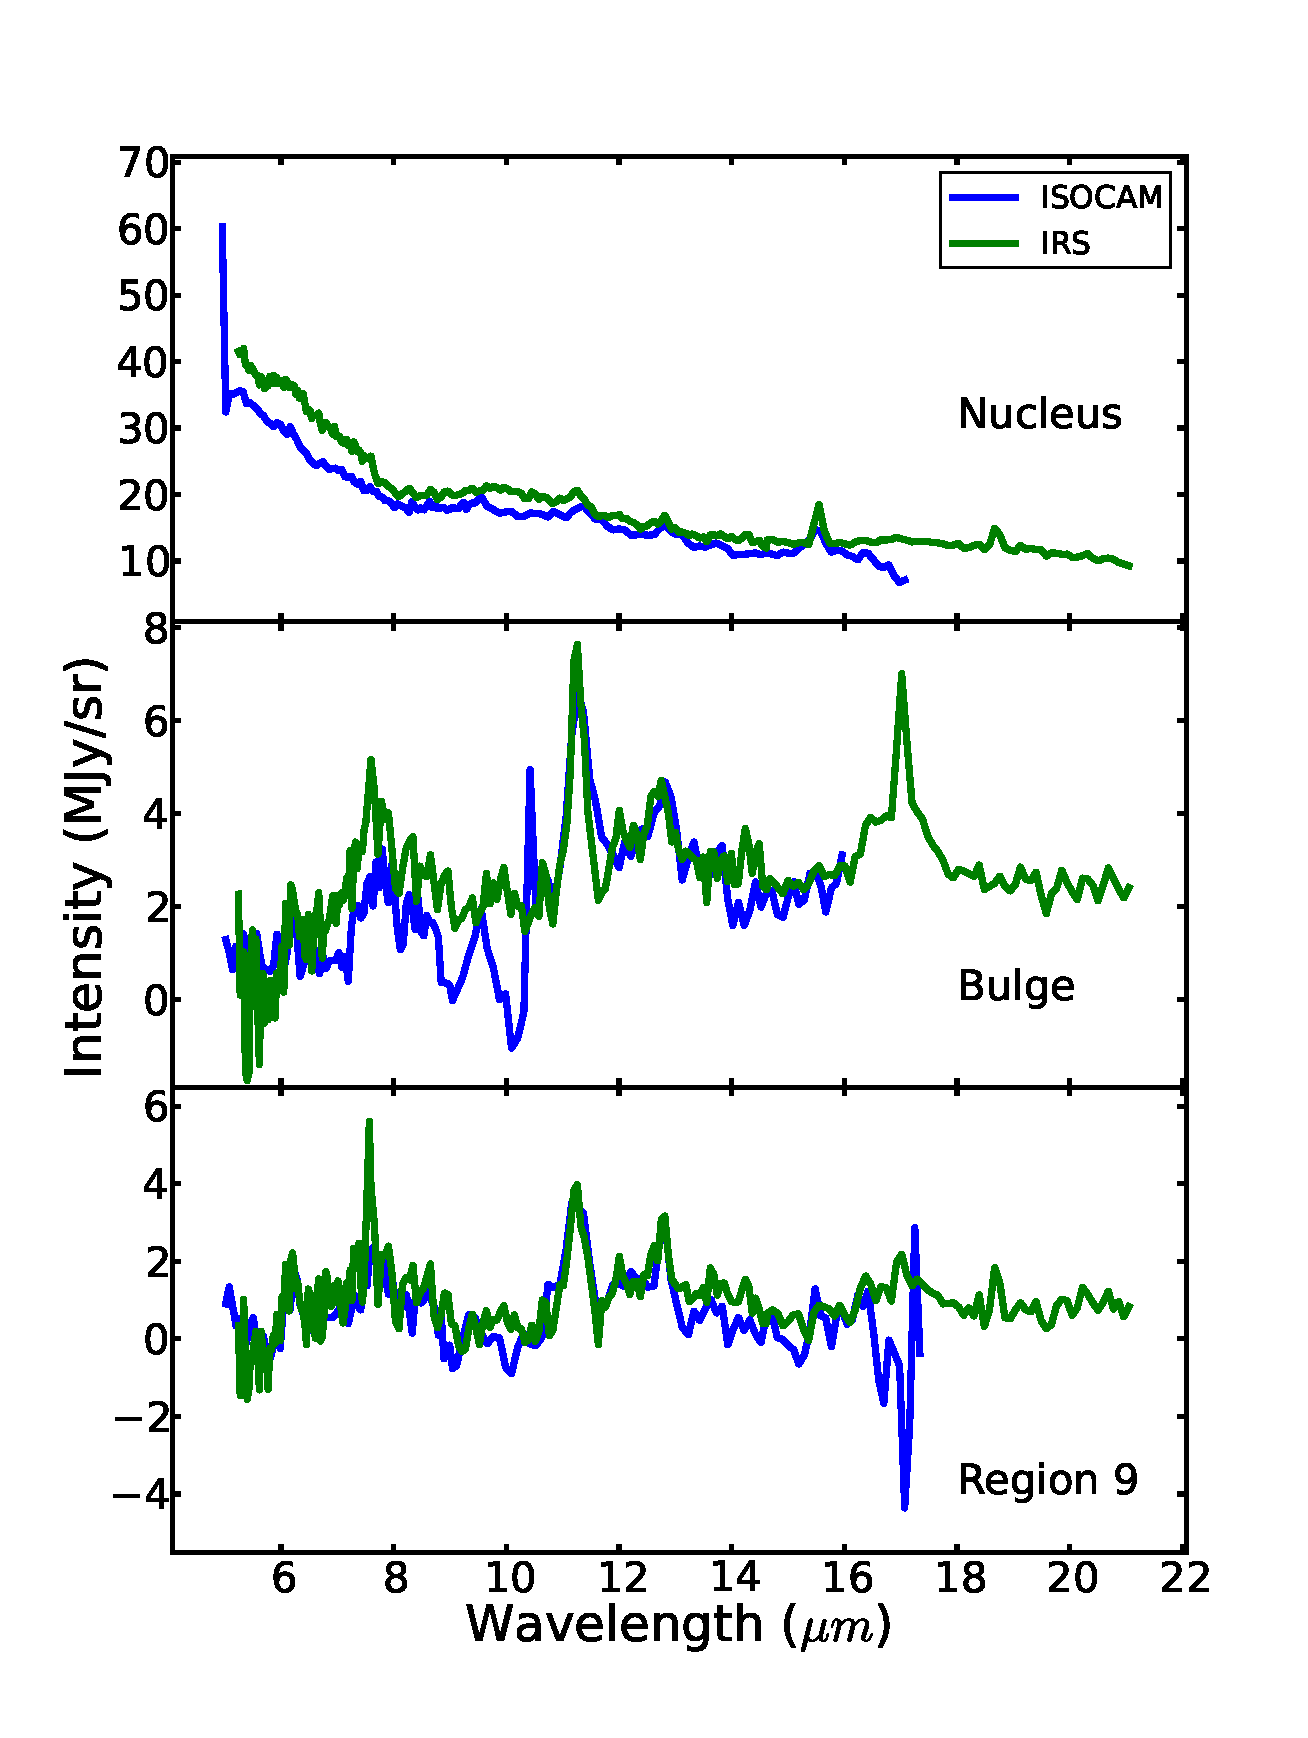
\includegraphics[scale=0.35]{./ISOvsIRS.eps}
\caption{ Comparison of  IRS and re-processed ISOCAM spectra for the Nucleus (top), Bulge (middle) and Region 9 (bottom) in M31.}
\label{ISOnIRS}
\end{figure}


\subsection{PAHFIT}

The PAH features in the IRS spectra are often blended with neighbouring aromatic features and atomic lines. Therefore measuring the strength of PAH features is difficult. To achieve this task a tool called PAHFIT, introduced by \citet{Smith:2007lr}, was used. PAHFIT is an IDL  based tool designed for decomposing {\em Spitzer} IRS spectra of PAH emission sources and is capable of identifying PAH features among other blended features. It also takes silicate absorption and extinction into account. PAHFIT is primarily designed for use with full 5--35~$\mu$m {\em Spitzer} low-resolution IRS spectra.

PAHFIT uses six main components to fit the surface brightness. These are starlight continuum, featureless thermal dust continuum, pure rotational lines of H$_2$, fine-structure lines, dust emission features and dust extinction. The starlight is represented by a modified blackbody emission at a fixed temperature of 5000 K and the dust continuum is represented by 8 modified blackbodies at fixed temperatures of 35, 40, 50, 65, 90, 135, 200, and 300~K. However, the final fit obtained with PAHFIT does not necessarily take all dust continua into account. Line features are represented by Gaussian profiles and dust features are represented by Drude profiles. The infrared extinction is considered as a combination of a power law plus silicate features peaking at 9.7 and 18~$\mu$m. More details about PAHFIT can be found in \citet{Smith:2007lr}.


None of the IRS spectra shows a significant silicate absorption around 9.7 or 18~$\mu$m and the the extinction values calculated by PAHFIT were almost zero. Therefore, we adjusted the PAHFIT input parameters so that it does not take dust extinction into account. Except for the bulge, Region 5, Region 6 and Region 8, the spectra do not show much contribution from starlight. 
% MLNA: Why do you hard-wire these parameters to exclude them entirely, if there is *some* contribution seen from them in the spectra?
Therefore, the starlight parameter in PAHFIT was also set to zero so that it does not take starlight into account except for the regions mentioned above. 
PAHFIT did not fit the spectrum from the nucleus properly. This was due to the silicate emission around 9.7~$\mu$m and therefore we did not use PAHFIT data from the nucleus for our analysis.

% SPW: "Observed IRS spectra and detailed PAHFIT decompositions. Regions are labeled in each panel.  Black squares show the observed data, and ....  Vertical scales differ in different panels."  (Modify that last sentence as appropriate.)
% SPW: I'm not sure what the right-hand "Relative Extinction" scale is supposed to be, but if you keep it, explain it in the caption.
% SPW: Why are there multiple red lines (dust continuum) in some panels?
\begin{figure*}
\centering
\includegraphics[scale=0.45]{./ALL.eps}
  \caption{The spectra from 10 regions (black squares) shown with their detailed PAHFIT decomposition. Red, blue, light blue, pink and green lines represent the dust continua, PAH features, atomic lines, starlight continuum and the fit respectively. The black line shows the total continuum. Spectra from the nucleus and NGC 206 are not shown here.}
\label{PAHFITplots}
\end{figure*}


\subsection{PAH features}
\label{sect:pah}

PAHFIT returns fluxes and equivalent widths (EQWs) of PAH features which are given in Tables~\ref{PAHlinetable} and \ref{EQW}. The intensities of the features do not include any contribution from the continuum but the equivalent width computed by
\begin{equation}
{\rm EQW}=\int \frac{I_{\nu} - I_{\nu, {\rm cont}}}{I_{\nu, {\rm cont}}} \,d\lambda,
\end{equation}
is a measure of both the strength of the continuum emission ($I_{\nu, {\rm cont}} $) and the line strength ($I_{\nu,{\rm feature}}$). 
Here $I_{\nu} =I_{\nu,{\rm feature}}+ I_{\nu, {\rm cont}} $. 
The continuum emission is mainly coming from the dust grains. Hence, by studying EQWs of PAHs, we can study how the PAHs compete with the dust grains in the mid-IR wavelengths. Therefore the EQW values were obtained to analyze the characteristics of PAHs in M31. PAHFIT returns the EQW values for each PAH feature and the uncertainties were calculated using a Monte-Carlo method. In that method, for each region, PAHFIT was run 500 times on randomly generated data points  normally distributed within the uncertainties of the spectrum. PAHFIT returned 500 EQW values for each PAH feature and the standard deviation of EQWs for a given feature was taken as its uncertainty. 
The EQW values from IRC3 and ISOCVF regions were removed from our analysis because they have negative flux values in their spectra which can affect the EQWs. 
% TODO: change region names in above line


\subsection{Atomic line features}
\label{sect:atomic}

\begin{figure}
\centering
\includegraphics[scale=0.3]{./NevsS.eps}
\caption{ Log([Ne~{\sc iii}]/[Ne~{\sc ii}])  vs Log([S~{\sc iv}]/[S~{\sc iii}]) 18 for the M31 regions in our sample (black dots) and for the starburst sample from \citet{Engelbracht_2008} (open dots). The straight line is the line of best fit for the starburst sample.}
\label{SvsNe}
\end{figure}

PAHFIT also returns the emission line strengths and the flux uncertainties of atomic lines. These are listed in Table~\ref{Atomic}.
Line ratios of [Ne~{\sc iii}]/[Ne~{\sc ii}] and [S~{\sc iv}]/[S~{\sc iii}] 18 have been used as an indication of the radiation hardness. \citet{Engelbracht_2008} demonstrated that a combination of these two line ratios -which they call the radiation hardness index (RHI)- is a more sensitive indicator of the hardness of the radiation. The RHI values are calculated using
\begin{equation}
{\rm RHI} = \left( \log\frac{\textrm{[Ne~{\sc iii}] }}{\textrm{[Ne~{\sc ii}]}} + [0.71 + 1.58\log\frac{\textrm{{[S~{\sc iv}]}}}{\textrm{{[S~{\sc iv}]}}}\right) /2
\end{equation}
Here, 1.58 and 0.71 are the slope and the intercept of the [Ne~{\sc iii}]/[Ne~{\sc ii}]  vs [S~{\sc iv}]/[S~{\sc iii}] 18 plot (Figure \ref{SvsNe}) for the starburst sample from 
\citet{Engelbracht_2008}. The RHI has also been used by \citet{Gordon:2008lr} for M101 observations. To investigate whether the atomic line emission from the selected regions of M31 with the fit parameters described above, we compared them to the starburst sample (Figure \ref{SvsNe}). 
	
We calculated upper limits for non-detected lines \footnote{To find the upper limits for the flux of missing atomic lines, we assumed the line to be a 
Gaussian profile with a FWHM as given by PAHFIT. The peak intensity was taken to be 3 times the RMS, where RMS is the root mean square of 
the noise at the position of a missing line.}. Figure \ref{SvsNe}  shows that the limits are reasonably following the trend for the starburst galaxy sample. 
Therefore the equation mentioned above was adopted with a simple modification to calculate the RHI values for our sample. For the regions with missing Ne lines, 
equation~\ref{eq:s} was used and for the regions with missing S lines, equation~\ref{eq:ne} was used. 
\begin{equation}
{\rm RHI} = 0.71 + 1.58\log\frac{\textrm{[S~{\sc iv}]}}{\textrm{[S~{\sc iii}]}}
\label{eq:s}	
\end{equation}
\begin{equation}
{\rm RHI} = \log\frac{\textrm{[Ne~{\sc iii}]}}{\textrm{[Ne~{\sc ii}]}}
\label{eq:ne}	
\end{equation}
For Regions 2, 5, and 8, we used the upper limit values of their atomic line intensities to calculated RHI values.


\section{Results and Discussion}


\subsection{PAH band ratios}
\label{sect:pah_ratios}

Both the 6.2 and 7.7~$\mu$m features are thought to be coming from ionized PAHs and the 11.3~$\mu$m feature from neutral PAHs. Therefore we expect to see a correlation between the intensities of 6.2 and 7.7~$\mu$m PAH features normalized by the 11.3~$\mu$m feature.  Figure \ref{PAHlines}  compares the PAH flux ratios of 7.7/11.3  and 6.2/11.3 features. The figure shows a good correlation between these two PAH line ratios, consistent with that of the SINGS sample shown by \citet{Smith:2007lr}.
A similar correlation was also reported by  \citet{Galliano2008} for a sample of galaxies and a handful of extended H{\sc ii} regions
and by \citet{Vermeij2002} for Galactic and Magellanic Cloud H{\sc ii}regions. This provides evidence that the PAH emission from M31 is not unusual. 


\begin{figure}
\centering
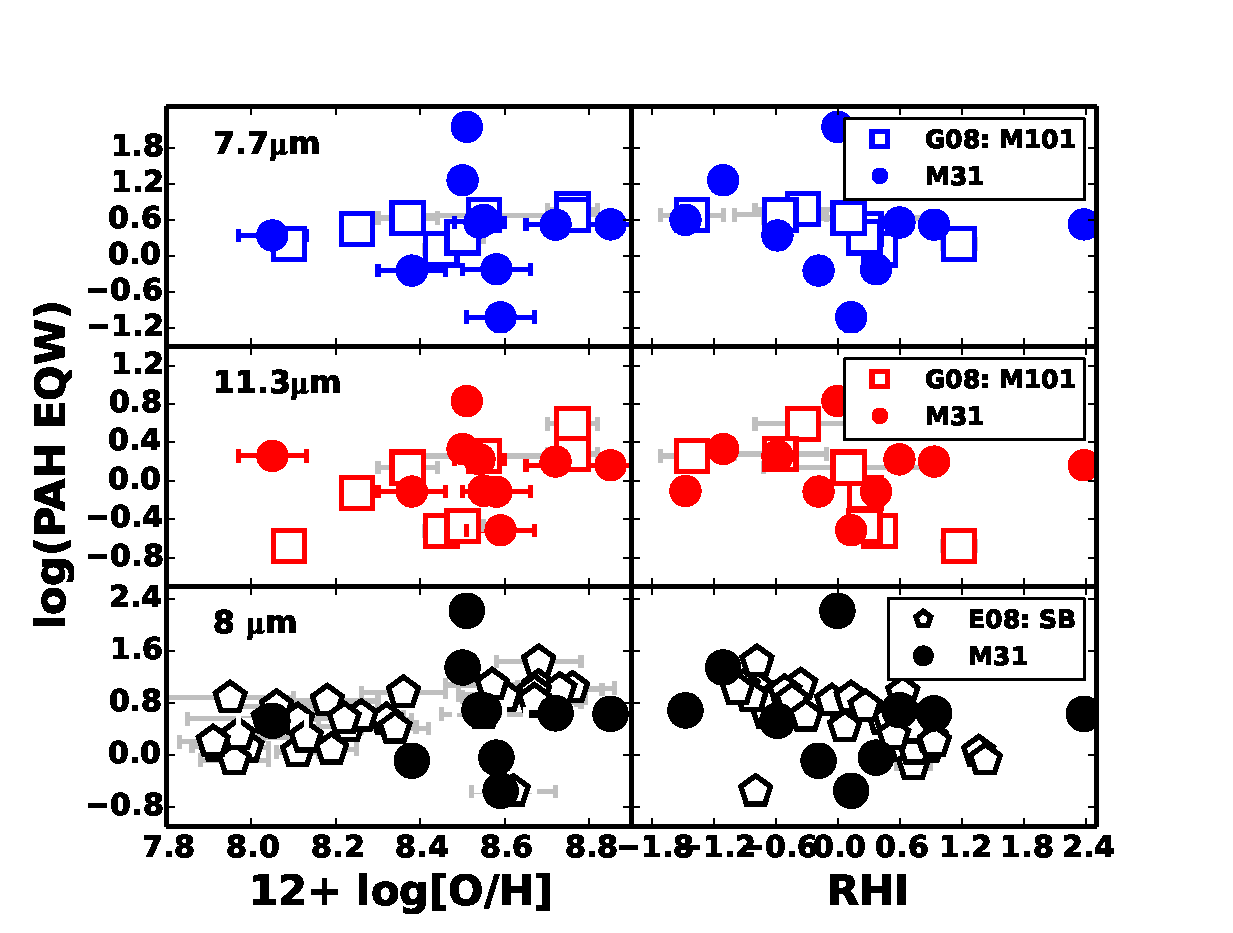
\includegraphics[scale = 0.25]{./fig9.eps}
\caption{Ratios of PAH feature fluxes (7.7~$\mu$m/11.3~$\mu$m versus 6.2~$\mu$m/11.3~$\mu$m) for 10 regions in M31.
Open squares represent the central regions of nearby galaxies as observed in the SINGS sample by \citet{Smith:2007lr}.
}
\label{PAHlines}
\end{figure}


\subsection{PAH equivalent widths versus radiation hardness and metallicity}
\label{sect:eqw_rh}

As mentioned in the introduction, PAH equivalent widths tend to decrease as radiation hardness increases,
and as metallicity decreases \citep{Calzetti:2010fk}.  
Figures~\ref{englII} and \ref{gordII} show the equivalent widths of the  8~$\mu$m feature 
(a combination of the 7.7, 8.3 and 8.6~$\mu$m PAHFIT components) and the 
 7.7 and 11.2~$\mu$m features as a function of RHI, with the starburst sample of \citet{Engelbracht_2008} 
and  H~{\sc ii} regions in M101 \citep{Gordon:2008lr} for comparison.
The M31 regions have about the same properties as the starburst galaxies and M101 H{\sc ii} regions, 
except for one M31 region with really high RHI (CHECK prob bad data) and one with really high EQW (CHECK).
No clear trend is defined by the M31 data, unsurprising given the uncertainties and the limited
number  of regions.
Figure \ref{metalicityVseqw} compares  PAH EQWs  versus  metallicity for our sample and the starburst 
galaxies of \citet{Engelbracht_2008} ( see also alternate version using Gordon data instead). 
We do not have enough data from low-metallicity regions in M31 to observe the expected decrease of PAH EQW with decreasing 
metallicity; however the M31 data occupy the same region of parameter space as the M101 data
and we conclude that the EQWs of the regions in M31 are consistent with previously published ``normal'' values.
The M31 region with very low  7.7~$\mu$m  equivalent widths is Region 8, which has
a noisy spectrum in the blue as well as substantial modelled contribution from starlight (see Figure~\ref{PAHFITplots}).


% combine following figures
\begin{figure}
\centering
\includegraphics[scale=0.4]{./fig10_new.eps}
\caption{Equivalent width of the 8~$\mu$m PAH feature versus radiation hardness index (RHI) for the M31 sample (blue),
and the starburst galaxy sample from \citet{Engelbracht_2008} (open squares).
}
\label{englII}
\end{figure}

\begin{figure}
\centering
\includegraphics[scale=0.30]{./fig11_new.eps}
\caption{Equivalent widths of the 7.7~$\mu$m PAH feature (top panel) and 11.3~$\mu$m PAH feature (bottom panel) versus 
radiation hardness index (RHI) for the M31 sample. Open squares represent H~{\sc ii} regions in M101 observed  by \citet{Gordon:2008lr}.  
}
\label{gordII}
\end{figure}

\begin{figure}
\centering
\includegraphics[scale=0.32]{./fig12_new.eps}
\caption{ PAH equivalent widths versus metallicity. 
Filled circles are M31 7.7~$\mu$m EQWs; filled squares are M31 11.3~$\mu$m EQWs; 
open circles are 8~$\mu$m EQWs for the starburst sample from \citet{Engelbracht_2008}.
Metallicities of the M31 regions have had 0.35~dex subtracted to account for the offset  between direct and strong-line measurements. 
}
\label{metalicityVseqw}
\end{figure}

\begin{figure}
\centering
\includegraphics[scale=0.4]{./fig12a.eps}
\caption{ PAH equivalent widths versus metallicity. 
Filled circles are M31 EQWs;  open squares are M101 EQWs from \citet{Gordon:2008lr}.
Metallicities of the M31 regions have had 0.35~dex subtracted to account for the offset  between direct and strong-line measurements. 
}
\label{metalicityVseqw}
\end{figure}





\section{Summary and Conclusions}

We  obtained {\em Spitzer}/IRS spectral maps of 12 regions within M31 covering wavelengths 5--21~$\mu$m. 
The spectra from those regions, except for the nucleus, are similar to spectra obtained from other nearby  star-forming galaxies. 
Early  ISOCAM observations  towards 4 regions of M31 showing a suppression 
of the 6--8~$\mu$m features and an enhancement of  the 11.3~$\mu$m feature  \citep{1998Cesarsky} 
were likely affected by the background subtraction methods applied.

The PAH intensities in M31 regions show a decreasing trend with increasing radiation hardness, consistent with previous 
results from other nearby galaxies. The distribution of PAH EQWs with metallicity is well within the range of the starburst galaxy sample of \citet{Engelbracht_2008}. 
We did not have enough data from low-metallicity regions of M31 to observe the decreasing trend of EQWs at low metallicities which is visible in other galaxies.

%SPW suggests separating on/off.
Mid-infrared spectra from near the nucleus of M31 show either suppressed 6--8~$\mu$m features and a strong 11.3~$\mu$m feature
(off-nucleus, GIVE DISTANCE) or silicate emission around 9.7~$\mu$m  (on-nucleus). 
The off-nucleus region spectrum is similar to that of six other nearby galaxies known to have low-luminosity AGN activity. This could strengthen the
suggestion by \citet{Smith:2007lr} that low $L(7.7\mu{\rm m})/L(11.3\mu{\rm m})$ is an indicator of low luminosity AGN,
but this feature ratio could also be due to a lack of ionized PAHs. The nuclear silicate emission is another possible AGN indicator. 
% UGH! Do something with this last setence.  
 

\section*{Acknowledgements}


DH acknowledges D. Stock, K. Sandstrom and S. Lianou for fruitful discussions and technical support. 
We acknowledge support from NSERC Discovery Grants to PB and EP and an NSERC Discovery Accelerator Grant to EP. 
This work is based on observations made with the {\em Spitzer} Space Telescope, which is operated by the 
Jet Propulsion Laboratory, California Institute of Technology under a contract with NASA.
This research has made use of NASA's Astrophysics Data System.



\bibliographystyle{mn2e}
\bibliography{reference}{}

\bsp

\label{lastpage}

\end{document}
